\documentclass[handout]{ximera}
\input{../../preamble}

\title{Area between curves}

\begin{document}
\begin{abstract}
  We compute the area of a region between two curves using the
  definite integral.
\end{abstract}
\maketitle


We have seen how integration can be used to find signed area between a
curve and the $x$-axis. With very little change we can find areas
bounded between curves.  Generally we should interpret ``area'' in the
usual sense, as a necessarily positive quantity. Suppose $f(x)>g(x)$
for all $x$ on the interval $[a,b]$ and we wish to know the geometric
area bounded between $f$ and $g$ on this interval:
\begin{image}
\begin{tikzpicture}
	\begin{axis}[
            domain=.5:2.5, ymax=10,xmax=2.5,ymin=0, xmin=.5,
            axis lines =left, xlabel=$x$, ylabel=$y$,
            xtick={1,2},
            ytick style={draw=none},
            width=4in,
            height=2in,
            yticklabels={},
            xticklabels={$a$, $b$},
            every axis y label/.style={at=(current axis.above origin),anchor=south},
            every axis x label/.style={at=(current axis.right of origin),anchor=west},
            axis on top,
          ]
          \addplot [draw=none,fill=fillp,domain=1:2] {-x^2+4*x+3} \closedcycle;
          \addplot [draw=none,fill=background,domain=1:2] {-x^3 + 7*x^2-10*x+5} \closedcycle;
          \addplot [draw=penColor,very thick] {-x^2+4*x+3};
          \addplot [draw=penColor2,very thick] {-x^3 + 7*x^2-10*x+5};
          \node at (axis cs:1,6.7) [penColor] {$f$};
          \node at (axis cs:2,4) [penColor2] {$g$};
        \end{axis}
\end{tikzpicture}
\end{image}
From the graph above we see that the area we want is the area under
$f$ minus the area under $g$, which is to say
\begin{align*}
\mathrm{Area} &= \int_a^b f(x)\d x-\int_a^b g(x)\d x \\
&= \int_a^b f(x)-g(x) \d x.
\end{align*}

We can also think of this ``infinitesimally'':

 In this case we are summing rectangles of
width $\d x$ and height $f(x)-g(x)$:
\begin{image}
\begin{tikzpicture}
	\begin{axis}[
            domain=.5:2.5, ymax=10,xmax=2.5,ymin=0, xmin=.5,
            axis lines =left, xlabel=$x$, ylabel=$y$,
            xtick={1,2}, yticklabels={},
            ytick style={draw=none},
            xticklabels={$a$, $b$},
            width=4in,
            height=2in,
            every axis y label/.style={at=(current axis.above origin),anchor=south},
            every axis x label/.style={at=(current axis.right of origin),anchor=west},
            axis on top,
          ]
          %\addplot [draw=none,fill=fillp,domain=1:2] {-x^2+4*x+3} \closedcycle;
          %\addplot [draw=none,fill=background,domain=1:2] {-x^3 + 7*x^2-10*x+5} \closedcycle;
          \addplot [draw=penColor,very thick] {-x^2+4*x+3};
          \addplot [draw=penColor2,very thick] {-x^3 + 7*x^2-10*x+5};
          \node at (axis cs:1,6.7) [penColor] {$f$};
          \node at (axis cs:2,4) [penColor2] {$g$};
          \addplot [draw=penColor, fill = fillp] plot coordinates {(1.5,2.375) (1.6,2.375) (1.6, 6.84) (1.5,6.84) (1.5, 2.375)};
          
          \draw[decoration={brace,mirror,raise=.2cm},decorate,thin] (axis cs:1.5,2.7)--(axis cs:1.6,2.7);
          \node at (axis cs:1.55,1.25) {$\d x$};

          \draw[decoration={brace,raise=.2cm},decorate,thin] (axis cs:1.51,2.375)--(axis cs:1.51,6.84);
          \node[anchor=east] at (axis cs:1.45,4.6) {$f(x)-g(x)$};
        \end{axis}
\end{tikzpicture}
\end{image}
In this case, the integral
\begin{image}
  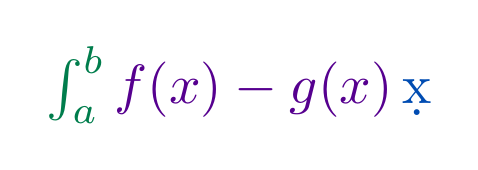
\begin{tikzpicture}[scale=2,every node/.style={transform shape}]
    \node at (0,0) {
      $\color{green!70!black!70!blue}\int_{a}^{b}\color{purple!50!blue!90!black}{f(x) - g(x)} \,\color{blue!70!green}{\d x}$
    };
  \end{tikzpicture}
\end{image}
could be interpreted as:
\begin{quote}
  \large\textbf{The \textcolor{green!70!black!70!blue}{sum} of the
    area of rectangles whose
    \textcolor{purple!50!blue!90!black}{heights are the difference
      between the top curve and bottom curve}, and whose
    \textcolor{blue!70!green}{widths are infinitesimal}.}
\end{quote}

\section{Integrating with respect to \textit{x}}

We'll start with basic examples and gradually build to more difficult
ones.

\begin{question}
  Let $f(x) = -x^2+4x+3$ and $g(x)=-x^3+7x^2-10x+5$. Compute the area
  between them on the interval $1 \le x \le 2$.
  
  	\begin{itemize}
  		\item Draw a picture, including the infinitesimal rectangle
  		\item Set up the definite integral
  		\item Evaluate the definite integral
  	\end{itemize}
  	
\newpage
\end{question}



In our first example, one curve was higher than the other over the
entire interval. This does not always happen.

\begin{question} 
Find the area between $f(x)= -x^2+4x$ and
$g(x)=x^2-6x+5$ over the interval $0 \le x \le 1$.

\newpage
\end{question}


In both of our examples above, we gave you the limits of integration
by bounding the $x$-values between $0$ and $1$. However, in some problems
you will have to do more work to determine these bounds.

\begin{question}
Find the area bounded between $f(x)= -x^2+4x$ and $g(x)=x^2-6x+5$.
\begin{image}
\begin{tikzpicture}
	\begin{axis}[
            domain=0:5, ymax=5,xmax=5,ymin=-5, xmin=0,
            axis lines =center, xlabel=$x$, ylabel=$y$,
 	   xtick={0.5635},
            xticklabels={$a$}, 
            every axis y label/.style={at=(current axis.above origin),anchor=south},
            every axis x label/.style={at=(current axis.right of origin),anchor=west},
            axis on top,
          ]
          \addplot [draw=none,fill=fillp,domain=.56:4] {-x^2+4*x} \closedcycle;
          \addplot [draw=none,fill=fillp,domain=.56:4.44] {x^2-6*x+5} \closedcycle;
          \addplot [draw=none,fill=background,domain=4:5] {-x^2+4*x} \closedcycle;
          \addplot [draw=none,fill=background,domain=0:1] {x^2-6*x+5} \closedcycle;
          %\addplot [draw=none,fill=fillp,domain=.56:4] {-x^2+4*x} \closedcycle;       
          \addplot [draw=penColor,very thick,smooth] {-x^2+4*x};
          \addplot [draw=penColor2,very thick,smooth] {x^2-6*x+5};
          
          \node at (axis cs:2,4.4) [penColor] {$f$};
          \node at (axis cs:1,-1) [penColor2] {$g$};
	 \node at (axis cs:4.43649,0.3) [textColor] {b};
	 \addplot [textColor,dashed] plot coordinates {(0.5635,0) (0.5635,1.9364)};
          \addplot [textColor,dashed] plot coordinates {(4.43649,0) (4.43649,-1.9364)};
        \end{axis}
\end{tikzpicture}
\end{image}

\newpage
\afterpage{\null\newpage}

\end{question}

\section{Integrating with respect to \textit{y}}

Consider the region bounded by the function $f(x) = x-3$, $g(x) =
\sqrt{x-1}$ and the horizontal axis:
\begin{image}
\begin{tikzpicture}
	\begin{axis}[
            domain=0:5.5, ymax=2.5,xmax=5.5, ymin=0, xmin=0,
            axis lines =center, xlabel=$x$, ylabel=$y$,
            every axis y label/.style={at=(current axis.above origin),anchor=south},
            every axis x label/.style={at=(current axis.right of origin),anchor=west},
            axis on top,
          ]
          \addplot [ fill = fillp, smooth, samples=100, domain=(0:2)] ({1+x^2},{x}) \closedcycle;
          \addplot [draw=none,fill=background,domain=0:5.2] {x-3} \closedcycle;   
          \addplot [very thick, penColor2, smooth, samples=100, domain=(0:3)] ({1+x^2},{x});
          \addplot [draw=penColor,very thick,smooth] {x-3};
          
          \node at (axis cs:3.4,1.7) [penColor2] {$g$};
          \node at (axis cs:4,0.7) [penColor] {$f$};
        \end{axis}
\end{tikzpicture}
\end{image}

While we could find the area of this region by breaking the
computation up into the two regions $[1,3]$ and $[3,5]$ (check that
$5$ is the intersection point!), there is another approach.  We can
think of splitting the region up into \textbf{horizontal} rectangles.

We can rewrite $y = \sqrt{x-1}$ as $x = y^2+1$, and we can rewrite $y
= x-3$ as $x = y+3$, so we have the following picture:

\begin{image}
\begin{tikzpicture}
	\begin{axis}[
            domain=0:5.5, ymax=2.5,xmax=5.5, ymin=0, xmin=0,
            axis lines =center, xlabel=$x$, ylabel=$y$,
            every axis y label/.style={at=(current axis.above origin),anchor=south},
            every axis x label/.style={at=(current axis.right of origin),anchor=west},
            axis on top,
          ]
          %\addplot [ fill = fillp, smooth, samples=100, domain=(0:2)] ({1+x^2},{x}) \closedcycle;
          %\addplot [draw=none,fill=background,domain=0:5.2] {x-3} \closedcycle;   
          \addplot [very thick, penColor2, smooth, samples=100, domain=(0:3)] ({1+x^2},{x});
          \addplot [draw=penColor,very thick,smooth] {x-3};
          
          \node at (axis cs:3.4,1.7) [penColor2] {$g$};
          \node at (axis cs:4,0.7) [penColor] {$f$};

	  \addplot [draw=penColor, fill = fillp] plot coordinates {(2,1) (2,1.1) (4, 1.1) (4,1) (2, 1)};

          \draw[decoration={brace,raise=.2cm},decorate,thin] (axis cs:2,1)--(axis cs:2,1.1);
          \node at (axis cs:1.6,1.05) {$\d y$};

          \draw[decoration={brace,mirror,raise=.2cm},decorate,thin] (axis cs:2,1)--(axis cs:4,1);
          \node at (axis cs:2.7,.7) {$f^{-1}(y)-g^{-1}(y)$};
        \end{axis}
\end{tikzpicture}
\end{image}
In this case, the integral
\begin{image}
  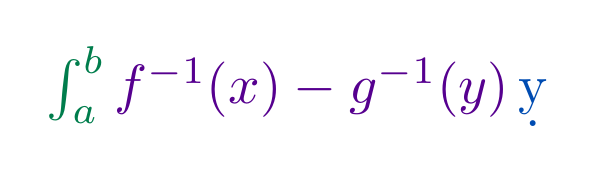
\begin{tikzpicture}[scale=2,every node/.style={transform shape}]
    \node at (0,0) {
      $\color{green!70!black!70!blue}\int_{a}^{b}\color{purple!50!blue!90!black}{f^{-1}(x) - g^{-1}(y)} \,\color{blue!70!green}{\d y}$
    };
  \end{tikzpicture}
\end{image}
could be interpreted as:
\begin{quote}
  \large\textbf{The \textcolor{green!70!black!70!blue}{sum} of the
    area of rectangles whose
    \textcolor{purple!50!blue!90!black}{widths are the difference
      between the right curve and left curve}, and whose
    \textcolor{blue!70!green}{heights are infinitesimal}.}
\end{quote}

Let's finish this example:

\begin{example}
  Compute the area of the region bounded by the function $f(x) = x-3$,
  $g(x) = \sqrt{x-1}$ and the horizontal axis.
  \newpage
  \afterpage{\null\newpage}

\end{document}